\documentclass[a4paper,10pt]{article}
\usepackage[spanish,activeacute]{babel}
\usepackage[latin1]{inputenc}
\usepackage[T1]{fontenc}
\usepackage[pdftex]{color,graphicx}
\usepackage{fancyhdr}
\usepackage{amsmath}
\usepackage{listings}
\usepackage{float}
\usepackage{color}


\floatstyle{ruled}
\newfloat{code}{hbt}{lop}
\floatname{code}{Codigo}

\lstset{
  language=C,                     % choose the language of the code
  basicstyle=\tiny,                 % the size of the fonts that are used for the code
  numbers=left,                   % where to put the line-numbers
  numberstyle=\footnotesize,      % the size of the fonts that are used for the line-numbers
  stepnumber=1,                   % the step between two line-numbers. If it's 1 each line will be numbered
  numbersep=5pt,                  % how far the line-numbers are from the code
  backgroundcolor=\color{white},  % choose the background color. You must add \usepackage{color}
  showspaces=false,               % show spaces adding particular underscores
  showstringspaces=false,         % underline spaces within strings
  showtabs=false,                 % show tabs within strings adding particular underscores
  frame=tb,			% adds a frame around the code
  tabsize=2,			% sets default tabsize to 2 spaces
  captionpos=b,			% sets the caption-position to bottom
  breaklines=true,		% sets automatic line breaking
  breakatwhitespace=false,  	% sets if automatic breaks should only happen at whitespace
  escapeinside={\%*}{*)},         % if you want to add a comment within your code
  stringstyle=\ttfamily,
  numberstyle=\tiny,
  extendedchars=true,
  frameround=tftf,
  inputencoding=latin1,
  numberblanklines=false,
  keepspaces=true,
  prebreak = \raisebox{0ex}[0ex][0ex]{\ensuremath{\hookleftarrow}},
  keywordstyle=\color{blue},
  commentstyle=\color[rgb]{0.5,0.5,0.5},
  stringstyle=\color{red}
}


\newcommand{\tp}{Trabajo Pr\'actico N$^{\circ}$\numtp}
\newcommand{\?}{?`}


\pagestyle{fancy}
\renewcommand{\sectionmark}[1]{\markright{#1}{}}
\lhead{\includegraphics[width=7mm,height=7mm]{\logo} \materia}
\chead{}
\rhead{\nomtp}
\lfoot{\rightmark}
\cfoot{}
\rfoot{\thepage}
\renewcommand{\headrulewidth}{0.4pt}
\renewcommand{\footrulewidth}{0.4pt}
\renewcommand{\headheight}{24pt}


\renewcommand{\theenumii}{\arabic{enumii}}
\renewcommand{\labelenumii}{\theenumi.\theenumii}
\renewcommand{\theenumiii}{\arabic{enumiii}}
\renewcommand{\labelenumiii}{\theenumi.\theenumii.\theenumiii}


\begin{document}
%\documentclass[a4paper,11pt]{report}
%\usepackage[spanish,activeacute,es-notilde]{babel}
%\usepackage[latin1]{inputenc}
%\usepackage[T1]{fontenc}
%\usepackage[pdftex]{color,graphicx}


\newcommand{\materia}{Sistemas de Computaci\'on 2}
\newcommand{\team}{Grupo N$^{\circ}$63}
\newcommand{\comision}{3900}
\newcommand{\diacursada}{Miercoles}
\newcommand{\turno}{Noche (de 19 a 23 Hs.)}
\newcommand{\anio}{2010}
\newcommand{\fecha}{30/06/2010}
\newcommand{\numtp}{4}
\newcommand{\nomtp}{Fork, Procesos Concurrentes, Zombies y Exec}
\newcommand{\docentes}{Favio Rivalta | Juan Manuel Fera | Soledad \'Alvarez}
%Poner aca la ruta al logo de la universidad.
\newcommand{\logo}{/home/ric/Documentos/Facultad/Varios/logoUnlam.png}

%\begin{document}
\thispagestyle{empty}

\begin{center}

 \includegraphics{\logo}
 % logoUnlam.png: 558x567 pixel, 200dpi, 7.09x7.20 cm, bb=0 0 201 204
 

\huge{Universidad Nacional\\de la Matanza}\\
\end{center}


\begin{center}
\rule{30mm}{.1pt}\\
\huge{\materia}\\
\huge{Trabajo Pr'actico N$^{\circ}$\numtp\\\nomtp}\\
\rule[5mm]{30mm}{.1pt}\\
\end{center}
Comisi'on: \comision.\\
Dia de Cursada: \diacursada.\\
Docentes del Curso: \docentes.\\
Turno: \turno.\\
Fecha Entrega: \fecha.\\
Curso Lectivo: \anio.



\begin{center}

\Large{Integrantes del Grupo}\\
\rule[2.5mm]{15mm}{.1pt}\\

\begin{tabular}{r|r}
Ricardo Bevilacqua & 34.304.983\\
D\'{ }Aranno Facundo Nahuel & 34.842.320\\
Moure Pablo & 32.031.459\\
Marcela A. Uslenghi & 26.920.315
\end{tabular}



\end{center}
\newpage


%\end{document}


\setcounter{page}{1}
\pagenumbering{roman}
\tableofcontents
\newpage
\setcounter{page}{1}
\pagenumbering{arabic}

\section{Ejercicio 1}

\subsection{C'odigo}
\lstinputlisting[title=ej1.c]{../cod/ej1/ej1.c}
\hyphenation{si-guien-tes}
\subsection[Punto A]{\?Cu'antos hijos, nietos y bisnietos producen las siguientes l'ineas?}
Las lineas producen:
\begin{description}
 \item 1 hijo
 \item 1 nieto
 \item 1 bisnieto
 \item 1 tataranieto
\end{description}

L'ogicamente, tambi'en crea un padre.

\subsection[Punto B]{Graficar el 'arbol de salida.}
\begin{center}
 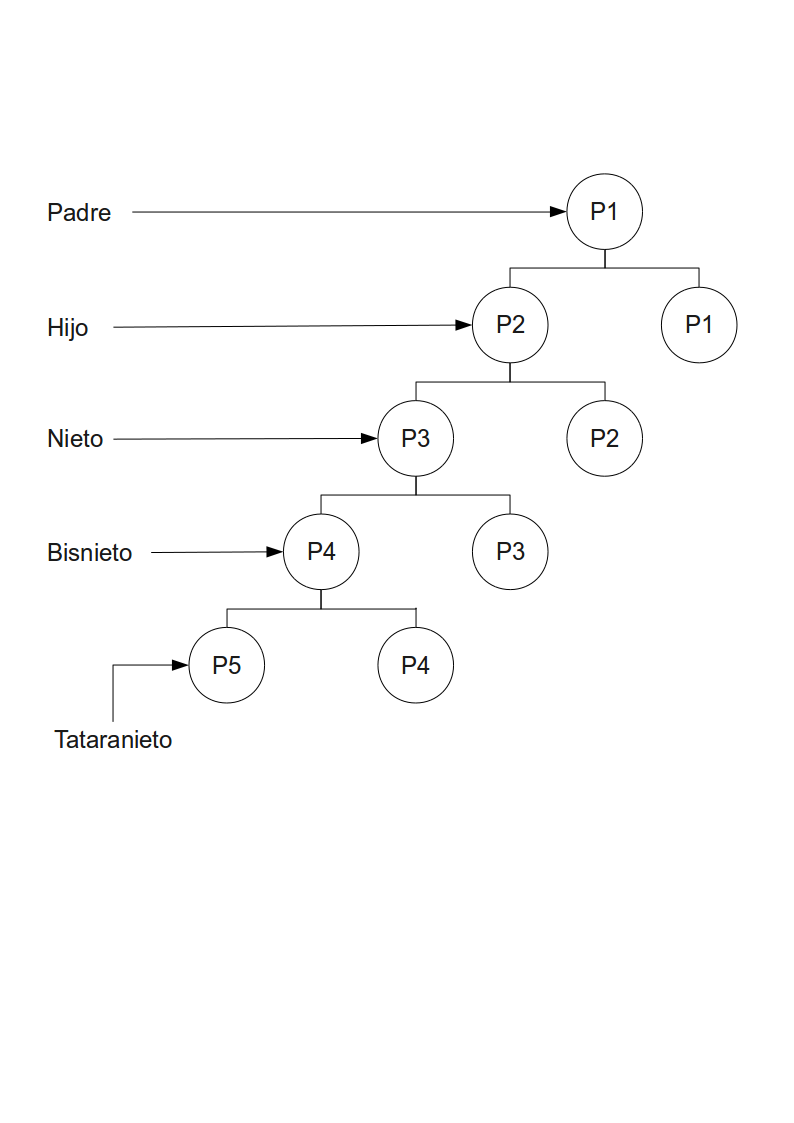
\includegraphics[scale=0.50,keepaspectratio=true]{./ej1/diagrama-ej1.png}
 % diagrama-ej1.png: 794x1123 pixel, 96dpi, 21.00x29.70 cm, bb=0 0 595 842
\end{center}


\subsection[Punto C]{Comentar el c'odigo.}
Ver c'odigo al principio.
\newpage
\subsection[Punto D]{Indicar que muestra cada mensaje, por qui'en es impreso y qu'e significado tiene,
c'omo se relacionan los mensajes entre s'i. Como parte de la soluci'on se debe
indicar un ejemplo de mensajes emitidos por el programa.}

\begin{lstlisting}
 $ ./ej1
  Mi PPID es 2417 y mi PID es 16233       (1)
  Mi PPID es 16233 y mi PID es 16234      (2)
  Mi PPID es 16233 y mi PID es 16234      (3)
  Mi PPID es 16234 y mi PID es 16235      (4)
  Mi PPID es 16235 y mi PID es 16236      (5)
  Mi PPID es 16234 y mi PID es 16235      (6)
  Mi PPID es 16235 y mi PID es 16236      (7)
  Mi PPID es 16236 y mi PID es 16237      (8)
\end{lstlisting}

Cada mensaje muestra el PID del padre y del hijo.

\begin{description}
 \item (1) Es impreso por el padre, su PPID es el PID del bash.
 \item (2) y (3) Es impreso por el hijo, su PPID es 16233, el padre.
 \item (4) y (6) Es impreso por el nieto, su padre es el proceso hijo 16234.
 \item (5) y (7) Es impreso por el bisnieto, su padre es el proceso nieto 16235.
 \item (8) Es impreso por el proceso tataranieto, su padre es el proceso nieto 16236.
\end{description}

\section{Ejercicio 2}

\subsection{C'odigo}
\lstinputlisting[title=ej2.c]{../cod/ej2/ej2.c}

\subsection[Punto A]{\?Qu'e proceso imprime el mensaje ``Fin!''?}
El mensaje ``Fin!'' es impreso por el proceso padre, en este caso ``ej2''.

\subsection[Punto B]{\?Por qu'e el mensaje ``Fin!'' es lo primero que se imprime? \?Qu'e sucede con el proceso hijo?}
Se imprime primero ``Fin!'' porque el padre termina antes que el hijo, el padre no espera al hijo a que termine. El proceso hijo es adoptado por el init, por quedar huerfano.

\subsection[Punto C]{\?C'omo se podr'ia solucionar?}
Se soluciona colocando un wait(NULL) antes del return del proceso padre.

\section{Ejercicio 3}

\subsection{C'odigo}
\lstinputlisting[title=ej3.c]{../cod/ej3/ej3.c}

\subsection{Errores}
Se encontraron 2 errores. Primero el compilador dio un aviso de la ausencia de la libreria stdlib.h por la funcion exit().
Segundo se noto que el padre terminaba antes que el hijo, la solucion fue agregar un wait(NULL) antes de que el padre informe que ha terminado.

\subsection[Punto A]{Note que para generar el hijo se utiliz'o la instrucci'on vfork. Indique por qu'e se realiz'o esto y cu'al es el prop'osito que se busca obtener.}
Se busca ejecutar el proceso de forma mas rapida no copiando todos los datos del PCB del padre, suspendiendo al padre hasta que el hijo ejecute un exec() o un \_exit().

\subsection[Punto B]{Tambi'en tenga en cuenta que luego de realizar el vfork no se realiza procesamiento de entrada salida, \?explique por qu'e?}
Una vez ejecutado en vfork() solo se puede llamar a una funcion de la familia exec() o \_exit().

\subsection[Punto C]{\?Por qu'e se utiliza la funci'on \_exit en lugar del exit tradicional?}
La funcion \_exit() se utiliza por lo mencionado en el punto b. \_exit() cierra la apicacion inmediatamente sin permitir otros parametros y validaciones que si permite el exit() tradicional.

\subsection[Punto D]{Documente que par'ametros utiliz'o para obtener una ejecuci'on correcta del c'odigo.}
Con especificar cualquier archivo ejecutable (este con o sin parametros) se logro la correcta ejecucion del ejercicio.

\section{Ejercicio 4}
\lstinputlisting[title=ej4.c]{../cod/ej4/ej4.c}

\section{Ejercicio 5}
\subsection{C'odigo}
\lstinputlisting[title=ej5.c]{../cod/ej5/ej5.c}

\subsection[Punto A]{\?Todos los hijos llegan al mismo n'umero en el acumulador? Justifique el comportamiento.}
No todos llegan al mismo n'umero en el acumulador ya que no todos terminan al mismo tiempo.

\subsection[Punto B]{Gr'aficos}
\begin{center}
 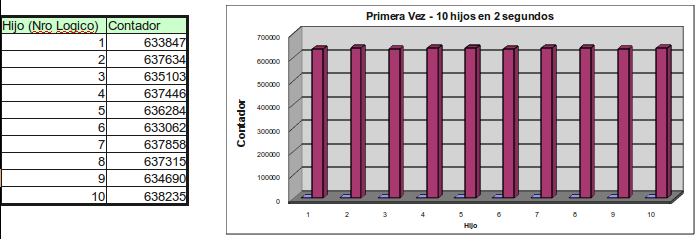
\includegraphics[scale=0.45,keepaspectratio=true]{./ej4/diag1.png}
 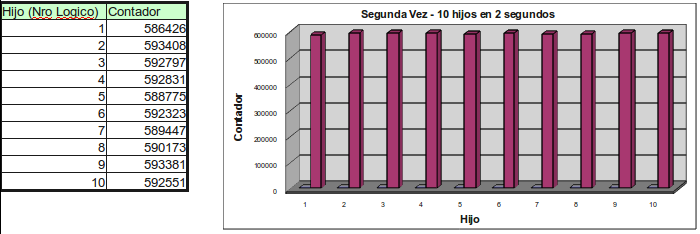
\includegraphics[scale=0.45,keepaspectratio=true]{./ej4/diag2.png}
 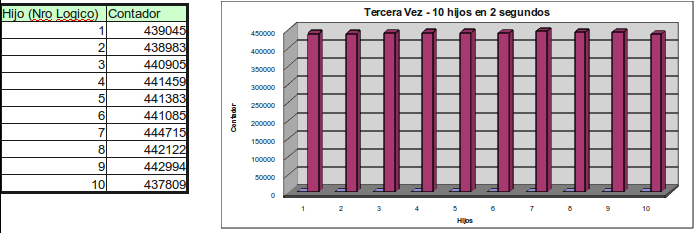
\includegraphics[scale=0.45,keepaspectratio=true]{./ej4/diag3.png}
\end{center}


\subsection[Punto C]{Analizando el gr'afico, \?es posible visualizar un patr'on de comportamiento? Explique.}
No es posible visualizar ning'un patr'on, ya que cada hijo termina en cualquier momento de forma aleatoria.

\section{Ejercicio 6}
\subsection{C'odigo}
\subsubsection{ej6.c}
\lstinputlisting[title=ej6.c]{../cod/ej6/ej6.c}
\subsubsection{split.h}
\lstinputlisting[title=split.h]{../cod/ej6/split.h}


\end{document} 
